
\RequirePackage{amsmath}
\DeclareMathOperator*{\argmax}{arg\,max}
\DeclareMathOperator*{\argmin}{arg\,min}
\documentclass{svjour3}
\usepackage{float}


\usepackage[margin=1in]{geometry}
\usepackage[numbers, sort&compress]{natbib}
\usepackage{pdfpages}
\usepackage{rotating}
\usepackage{relsize}
\usepackage{graphicx}
\usepackage{booktabs}
\usepackage[strings]{underscore}
\usepackage{anyfontsize}
\usepackage{subfig}
\usepackage{lipsum}
\usepackage[utf8]{inputenc}


\begin{document}

\abstract


\section{Introduction}
  
  
\section{Methodology}
The goal of the models presented in this paper is to predict the number of fires that occur in each census tract in the dataset over a five-year ``test" interval, comprising of the years 2012-2016 (inclusive). All models are strictly informed only by records that were completed prior to the end of the year 2011. This includes geocoded NFIRS data for residential fires that occurred the training interval, as well as the population, demographic, and housing unit information reported in the 2006-2010 American Community Survey 5-year estimates. Training the models using only data completed prior to the testing interval allows for the evaluation of the models' ability to make future predictions.


\section{Modeling overview}
The theoretical framework common to all models is that the occurrence of residential fires within each department follows a spatially inhomogeneous point process with an intensity function $\lambda_{i}(\textbf{x})$ 
where \textbf{x} is a point located in $\textbf{R}^2$ within the coverage area of department \textit{i}. $\Lambda_{i,j}$, described in equation \ref{eqn:rate_description}:

\begin{equation}
  \label{eqn:rate_description}
  \Lambda_{i,j} = \int_{B_{i,j}} \lambda_{i}(\textbf{x})d\textbf{x}
\end{equation}

\noindent where $B_{i,j}$ is the geographic area of census tract \textit{i,j}. Each of the models provides the estimated average rate of residential fires at the census tract level, $\hat\Lambda_{ij}$. Because this quantity is assumed to be temporally homogeneous\footnote{Note that in the most general sense, the intensity can also vary temporally such that $\lambda_i = \lambda_i(\textbf{x},t)$. Although the authors made various attempts to estimate the temporal evolution of $\lambda_i$, the large variance in the count data made it difficult to infer transient trends from the 6-year training interval that improve predictions relative to the assumption that $\lambda_i$ is temporally homogeneous.}, the prediction for the number of fires that occur during the test interval is then calculated according to equation \ref{eqn:rate_integral}: 

\begin{equation}
  \label{eqn:rate_integral}
  \hat{f}_{test,i,j} = \int_{0}^{n_{test}}\hat\Lambda_{i,j}dt
  = n_{test}\hat\Lambda_{i,j}
\end{equation}

\noindent where $n_{test}$ is the duration of the test interval (5 years) and $\hat{f}_{test,i,j}$ is the predicted number of fires that occur during the test interval.

Then the efficacy of a model's prediction is then quantified using the Poisson deviance, which is calculated according to equation \ref{eqn:deviance}:

\begin{equation}
  \label{eqn:deviance}
  D_i = 2\sum_{j=1}^{N_i}\bigg[
   f_{test,i,j}log\big(\frac{f_{test,i,j}}{\hat{f}_{test,i,j}}\big) - 
   (f_{test,i,j}-\hat{f}_{test,i,j}) 
  \bigg]
\end{equation}

\noindent where $N_i$ is the number of census tracts covered by department \textit{i}, $f_{test,i,j}$ is the number of residential fires that actually occurred in census tract \textit{i,j} during the 5-year test interval A lower deviance indicates more accurate predictions, with a deviance of zero corresponding to a model that perfectly predicted the number of residential fires that occurred in each census tract during the test interval.



\subsection{Utilizing spatial information}
The section outlines two purely spatial models that utilize only the locations of past fire in order to forecast future fire counts at the census tract level. The central assumption of these models is that fire risk factors are chronic, and proximity to previous fires indicates elevated risk to future fires. The first model is a naive ``spatial histogram'' model that serves as a performance baseline for all subsequent models described in this paper. The second employs Kernel Density Estimation (KDE), which is a statistical method commonly used to generate incident heatmaps. 

\subsubsection{Naive count forecasting (spatial histogram)}
The simplest forecasting technique described in this paper is a naive count model that can be thought of as a spatial histogram with the census tracts representing a set of non-uniform bins. The estimate for the count density rate in census tract \textit{j} covered by fire department \textit{i} is described by equation \ref{eqn:naive_count}:

\begin{equation}
  \label{eqn:naive_count}
  \hat{\Lambda}_{count,i,j} = \frac{f_{train,i,j}}{n_{train}} 
\end{equation}

\noindent where $\hat{\Lambda}_{count,i,j}$ is the estimated average fire density per year, $f_{train,i,j}$ is the total number of fires in census tract \textit{i, j} that occurred during the training interval, $n_{train}$ is the number of years that comprise the training interval (6 years), and $A_{i,j}$ is the land area of census tract \textit{i, j}. As an example, if 12 residential fires occurred in a census tract during the 6-year training interval (2 fires/year), then this framework would predict that 10 fires would occur in that census tract during the subsequent 5-year test interval. This methodology serves as a performance baseline for the more sophisticated forecasting models described later in this paper. An illustration of this methodology is provided in Figure \ref{fig:spatial_histogram}. 


\begin{figure}[htb] \centering
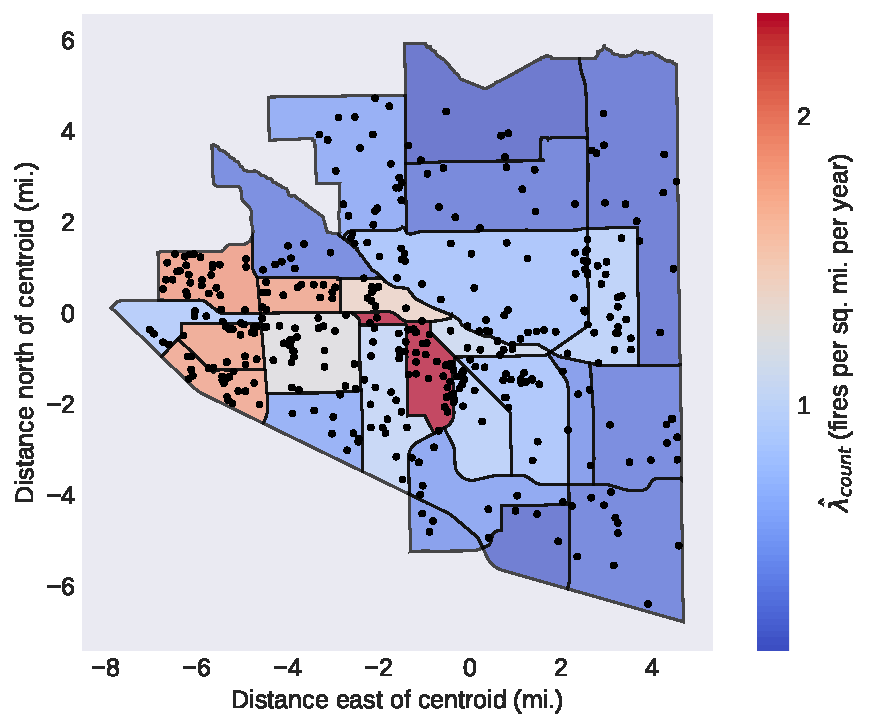
\includegraphics[width=.75\textwidth]{./figures/spatial_histogram.pdf}
\caption{A visual depiction of the naive count forecasting methodology for an example department. The black dot markers indicate the location of a residential fire that occurred during the six-year training interval, 2006-2011 (inclusive). The color corresponds to the fire count density rate estimated from this approach. Notice that large census tracts with few fires have the lowest density rate and small tracts with many fires have the highest density rate.}
\label{fig:spatial_histogram}
\end{figure}

\subsubsection{Kernel density estimation}
The second spatial model discussed in this paper is Kernel density estimation (KDE), which is a statistical methodology for inferring a density distribution from a set of point observations. This is the framework commonly used to generate incident heatmaps. The major difference between this method and the one outlined in the previous section is that KDE results  a smoothed surface that does not arise from ``binning" the incidents into discrete areas such as the census tract boundaries. Instead, this density surface is generated by centering a kernel function on each point (i.e. residential fire location) in the training set. The density function can then be calculated at any location by summing the kernel functions of all past residential fires at that location. This process is described by equation \ref{eqn:kde}:

\begin{equation}
  \label{eqn:kde}
  \hat\lambda_{i,KDE}(\textbf{x}) = \frac{1}{n_{train}}\sum_{m=1}^{F_i}K_i(\textbf{x},\tilde{\textbf{x}}_{i,m})
\end{equation}

\noindent where $F_i$ is the total number of fires that occurred during the training interval, and $\tilde{\textbf{x}}_{i,m}$ is the location of the $m^{th}$ residential fire that occured during the training interval in the coverage area of department \textit{i}. Note that the subscript \textit{j} is not used here because $\hat\lambda_{i,KDE}(\textbf{x})$ does not depend on census tract geometries. $K_i(\textbf{x},\tilde{\textbf{x}}_{i,m})$ is a department-specific kernel function. The KDE predictions described in this paper were obtained using a two-dimensional isotropic Gaussian kernel, described in equation \ref{eqn:gaussian_kernel}:


\begin{equation}
  \label{eqn:gaussian_kernel}
  K_i(\textbf{x},\tilde{\textbf{x}}_{i,m}) = \frac{1}{2\pi b_{i}^2}exp\bigg(\frac{d^2_i(\textbf{x},\tilde{\textbf{x}}_{i,m})}{2b_{i}^2}\bigg)
\end{equation}

\noindent where $d_i(\textbf{x},\tilde{\textbf{x}}_{i,m})= ||\textbf{x} - \tilde{\textbf{x}}_{i,m}||_2$, the euclidean distance between an arbitrary point \textbf{x} and $\tilde{\textbf{x}}_{i,m}$. $b_i$ is the department-specific bandwidth. Loosely speaking, it represents the length scale over which past fires elevate the estimated fire risk of surrounding areas. An important attribute of the kernel used in these analyses is that $\int_{\textbf{x} \in \textbf{R}^2}K_i(\textbf{x},\tilde{\textbf{x}}_{i,m})d\textbf{x} = 1$, and by extension, $n_{train}\int_{\textbf{x} \in \textbf{R}^2}\hat\lambda_{i,KDE}(\textbf{x}) d\textbf{x} = F_i$. In other words, the total kernel density is equal to the total number of fires that occurred during the training interval. In order to provide intuition for the reader, a simplified illustration of the KDE approach is provided in Figure \ref{fig:1dkde}.

\begin{figure}[htb] \centering
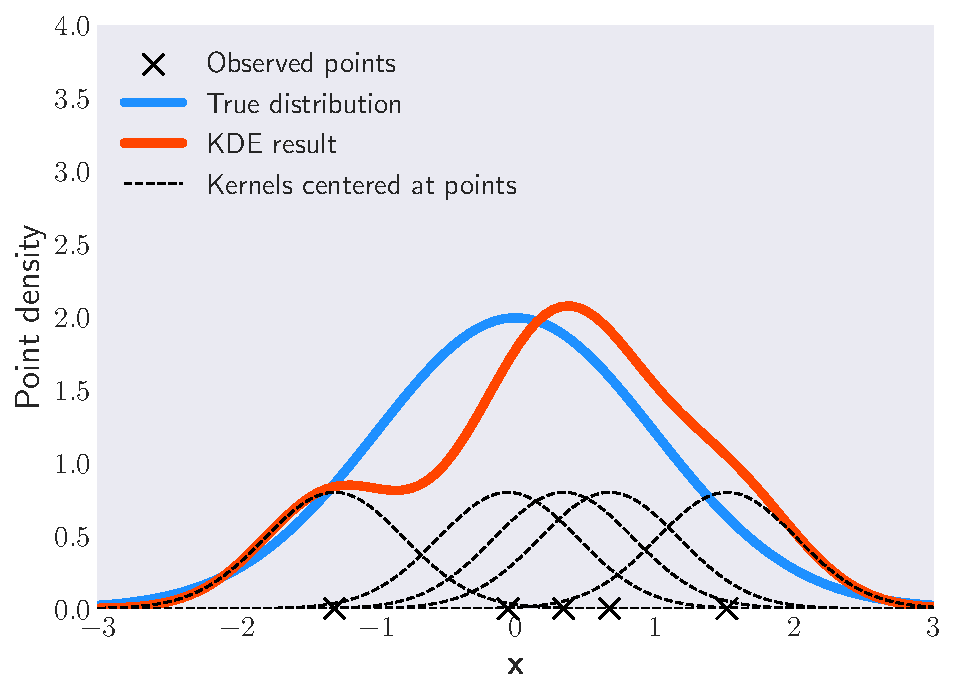
\includegraphics[width=.75\textwidth]{./figures/1dkde.pdf}
\caption{A simplified one-dimensional illustration of the KDE method. Although the locations of residential fires are defined in $\textbf{R}^2$, the use of a location coordinate defined in $\textbf{R}$ allows for an intuitive visualization. Five points (indicated by the ``X" markers) are drawn from a standard normal distribution, so that the true density function (the blue curve) is five times the standard normal probability distribution. The dashed black curves indicate Gaussian kernels centered on each point, and the red curve shows the KDE result, which is the sum of the kernels.}
\label{fig:1dkde}
\end{figure}

A key consideration for generating meaningful results from KDE is the selection of the bandwidth parameter, $b_i$. Selecting too small of a bandwidth results in density estimates that have highly localized peaks that correspond to the locations of past incidents; conversely, selecting too large of a bandwidth results in an overly smoothed density estimate that tends towards a uniform density profile as $b_i \rightarrow  \infty$. Figure \ref{fig:band_comparison} shows the effect of different bandwidth on the resulting KDE heatmaps along with the "optimized bandwidth" which is obtained through 5-fold cross validation. This technique randomly splits the training data into five groups of approximately equal size. Using a specific value for $b_i$, a KDE map is generated using the data from four of the five groups or folds. The algorithm then determines the likelihood of the the locations of the fires in the excluded fold using the map generated from incidents in the four remaining folds. This likelihood arises from the fact that $\frac{n_{train}}{F_i}\hat\lambda_{i,KDE}(\textbf{x})$ is actually an estimate of the probability density function for the location of a new fire. This process is then repeated so that each of the five folds are excluded, and 100 logarithmically spaced values of $b_i$ are evaluated over the interval $[0.01,10]$ miles and the bandwidth that generated KDE maps with the highest predictive accuracy is chosen as the optimal bandwidth, $b_{i,opt}$. This optimization process is described mathematically by equation \ref{eqn:fivefold}:

\begin{equation}
  \label{eqn:fivefold}
   b_{opt,i} = \argmax_{b_i} \prod_{k=1}^5 \prod_{m \in E_k}   \hat\lambda_{i,k}(\tilde{\textbf{x}}_m,b_i)
\end{equation}

\noindent where $\hat\lambda_{i,k}(\tilde{\textbf{x}}_m,b_i)$ is the KDE function that is generated using a bandwidth of $b_i$ and also excluding incidents in the k$^{th}$ fold, $E_k$. 

\begin{figure}[!ht]
       \begin{center}
  %
          \subfloat[$b_i=0.1$ mi]{%
              \label{fig:smallband} 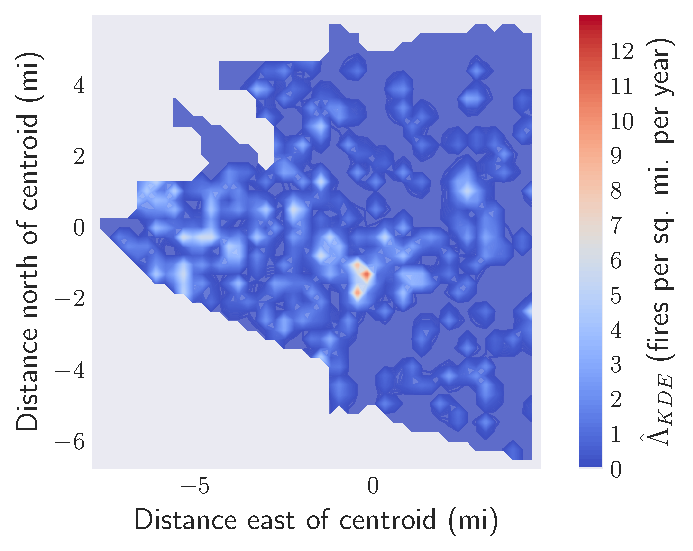
\includegraphics[width=.4\textwidth,keepaspectratio]{figures/small_band.pdf}
          }%
          \subfloat[$b_i= 1.0$ mi]{%
             \label{fig:largeband} 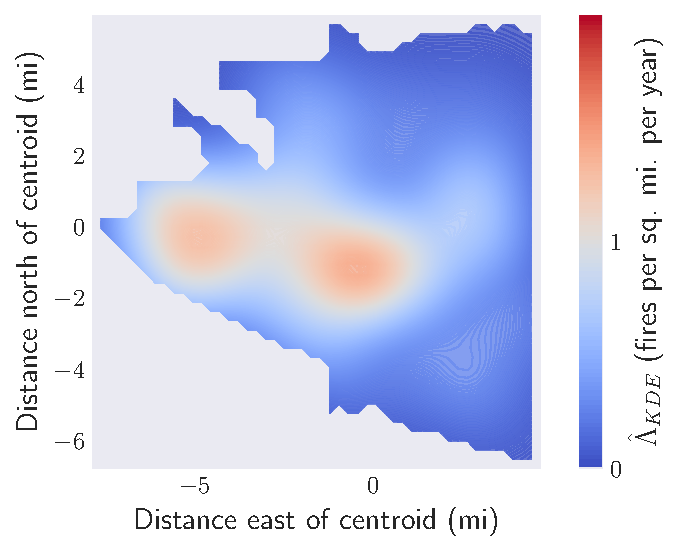
\includegraphics[width=.4\textwidth ,keepaspectratio]{figures/large_band.pdf}
          }\\ % 
            \subfloat[$b_i=b_{i,opt}=0.43$ mi]{%
             \label{fig:optband} 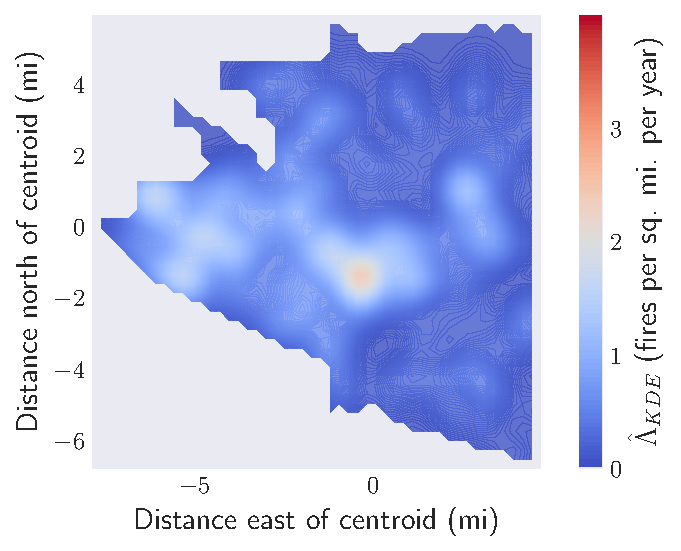
\includegraphics[width=.4\textwidth,keepaspectratio]{figures/correct_band.pdf}
          } % ------- End of the first row ----------------------%
      \end{center}
      \caption{ Visual depiction of the effect of different bandwidth values for heatmaps generated from KDE. The bandwidth is too small in \protect\subref{fig:smallband}, which is apparent from the many localized ``hotspots."  Conversely, the bandwidth is too large in \protect\subref{fig:largeband}, and the result is an overly smoothed heatmap. \protect\subref{fig:optband} shows the heatmap with the optimized bandwidth.}
     \label{fig:band_comparison}
  \end{figure}
  
 As previously indicated, the central idea of KDE is that proximity to past fires elevates the probability of future fires, and $b_opt$ is the distance that best specifies this proximity\footnote{Approximately 95\% of the kernel density from an incident is located within $2b_i$ of the incident location.} for predicting the locations of ``out of sample" fires. This means that the results obtained from the bandwidth optimizations give insight into the distances over which fire risk factors vary within the coverage areas of the departments in the dataset. Figure \ref{fig:bhist} shows that these distances vary significantly across departments, though $b_opt$ was between 0.1 and 0.4 miles for most departments. Furthermore, Figure \ref{fig:popband} reveals a negative correlation between $b_opt$ that explains some of the variation of $b_opt$ across the departments in the dataset. This result implies that residential fire risk factors spatially vary more significantly in communities with higher population densities than those with lower population densities. For example, knowledge of residential fires that occurred 0.75 miles away from a specific housing unit may elevate the probability of that unit experiencing a fire in regions of low population density, but less so in regions of high population density.

\begin{figure}[!ht]
       \begin{center}
  %
          \subfloat[Histogram of optimized bandwidths]{%
              \label{fig:bhist} 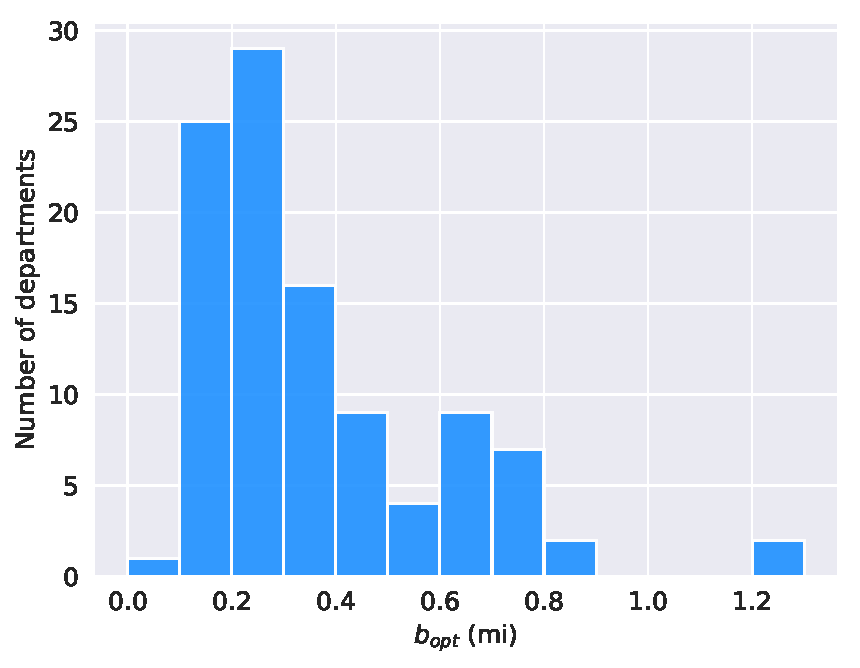
\includegraphics[width=.4\textwidth,keepaspectratio]{figures/optimal_band_dist.pdf}
          }%
          \subfloat[Scatterplot of optimized bandwidths vs. average department population density]{%
             \label{fig:popband} 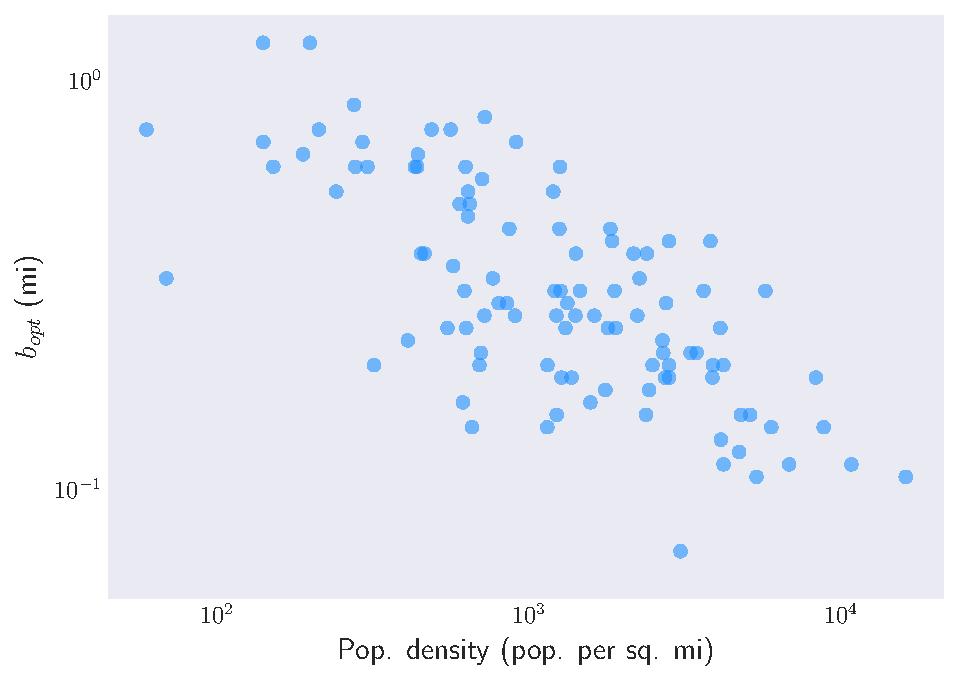
\includegraphics[width=.4\textwidth,keepaspectratio]{figures/boptvspopdensity.pdf}
          } % 
           % ------- End of the first row ----------------------%
      \end{center}
      \caption{\protect\subref{fig:bhist} shows the variation of the optimized bandwidth across departments in the dataset, and the negative correlation apparent in \protect\subref{fig:popband} shows that this variation is at least partially explained by the variation in population density across departments.}
     \label{fig:band_optimization}
  \end{figure}
  
  Calculating $b_{i,opt}$ for each department allows for the determination of $\hat\lambda_{i,KDE}(\textbf{x})$ according to equation \ref{eqn:kde}. The KDE estimate for the number of fires that occur during the test interval can then be obtained from equation \ref{eqn:rate_description}. However, because $\hat\lambda_{i,KDE}(\textbf{x})$ does not have an analytical form, the estimate is generated by evaluating it at a set of 100 by 100 evenly spaced grid points within each census tract and then performing a numerical integration. Note that this generates different estimates of  $\Lambda_{i,j}$ than using the spatial histogram approach because the kernel densities from individual fire incidents ``spill out" across census tract boundaries. In fact, The spatial histogram approach can be viewed as a special case of the KDE approach where $b_i \rightarrow 0$, which makes the kernels analagous to a set of Dirac delta functions in which the entire density is located at a point, but it still integrates to one.
  
  
  

  \subsection{Utilizing demographic and structural information}
  In contrast to the models presented in the previous section, the focus of this section is to utilize only the socio-demographic and structural information from the American Community Survey 5-year summary file (ACS5). In this section, the fire incident location data is used only to assign each incident to a census tract. After these assignments, the ACS5 data is the sole basis of the training features. This means that the location of census tracts relative to other census tracts is not incorporated into the model described in this section.

  \subsubsection{Feature visualization}
  Before desribing the model that utilizes ACS5 data, it is worth understanding the underlying relationships between the fire rates in census tracts and their structural and socio-demographic profiles. Perhaps the most intuitive starting point is the recoginition that residential fires occur where people live, so it is reasonable to expect a positive relationship between the rate of fires experienced by a census tract and its population. The authors found that normalizing these quantities by the census tract area improves the clarity of the relationship, which is shown in Figure \ref{fig:pop_relation}. It also allows for the delineation between urban and rural communities; as a rule of thumb, the Census Bureau   \cite{ratcliffe2016defining} uses a population density of 1,000 pop. per. sq. mile as a guideline for the cutoff between urban and rural for census blocks. Although the dataset is comprised of census tracts rather than blocks and this criterion serves as one component of the urban/rural designation, it still provides intuition for the separation between rural and urban communities, and as a result is chosen as the separating line in the figures. The relationship is fairly linear, which is the first trend that can be used to inform a predictive model.
    
     \begin{figure}[htb] \centering
    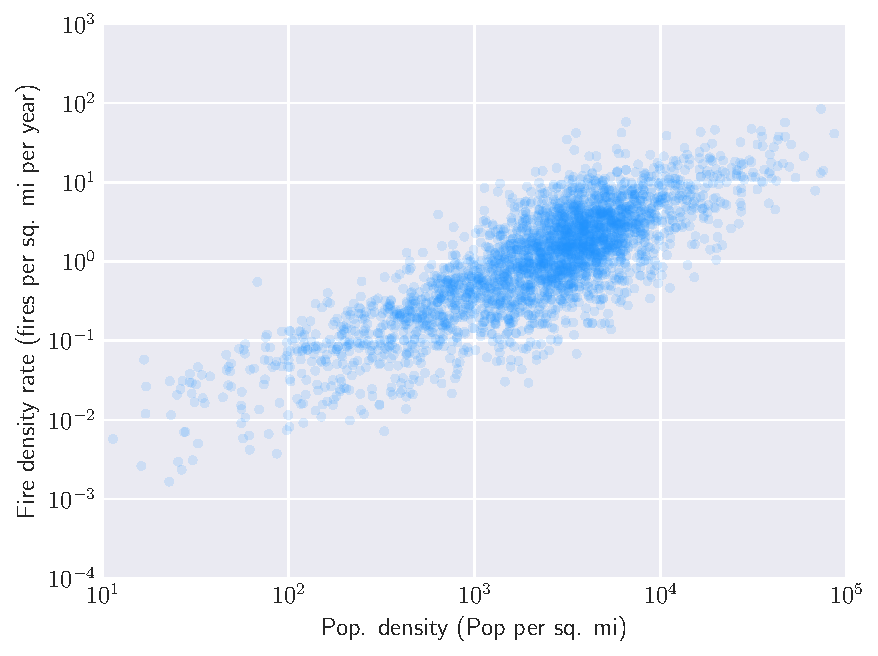
\includegraphics[width=.75\textwidth]{figures/pop_relation.pdf}
    \caption{A scatterplot of the observed fire count density rate during the training interval vs. population density ($\hat\Lambda_{count}$) for all 3,009 census tracts in the dataset. }
    \label{fig:pop_relation}
    \end{figure}
  
  In light of the linear relationship shown in Figure \ref{fig:pop_relation}, the effects of other socio-demographic factors that influence fire risk can be understood in terms of upward or downward ``shifts" to the approximately linear cloud of points representing census tracts. This also can be viewed as changes in the fire rate per person. This is shown in Figure \ref{fig:sociodemographic}.
  
  \begin{figure}[!ht]
       \begin{center}
  %
          \subfloat[Median income]{%
              \label{fig:median_income} 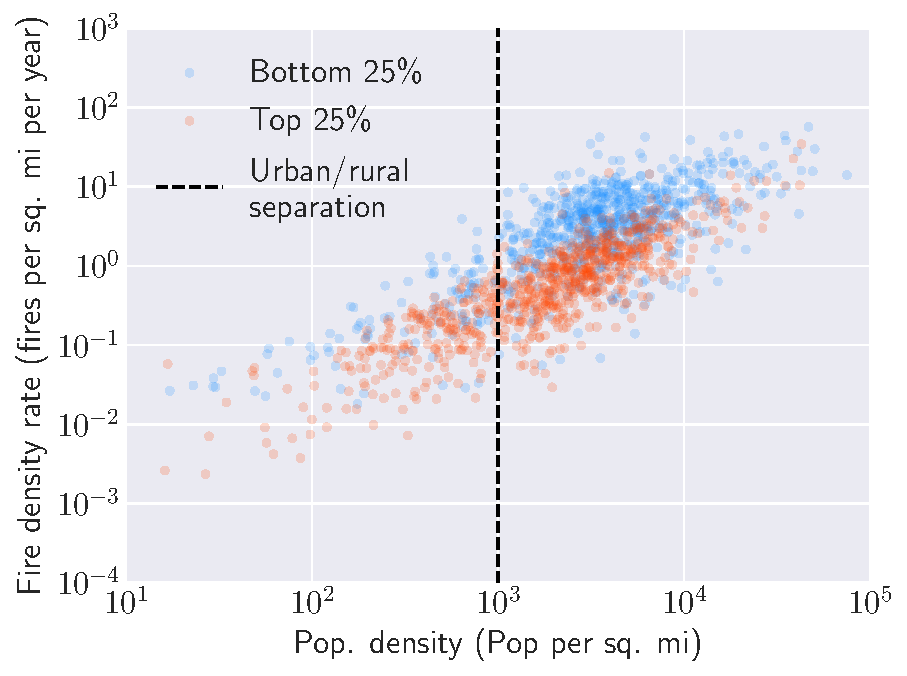
\includegraphics[width=.4\textwidth,keepaspectratio]{figures/median_income.pdf}
          }%
          \subfloat[Fraction of population holding college degrees]{%
             \label{fig:frac_degree} 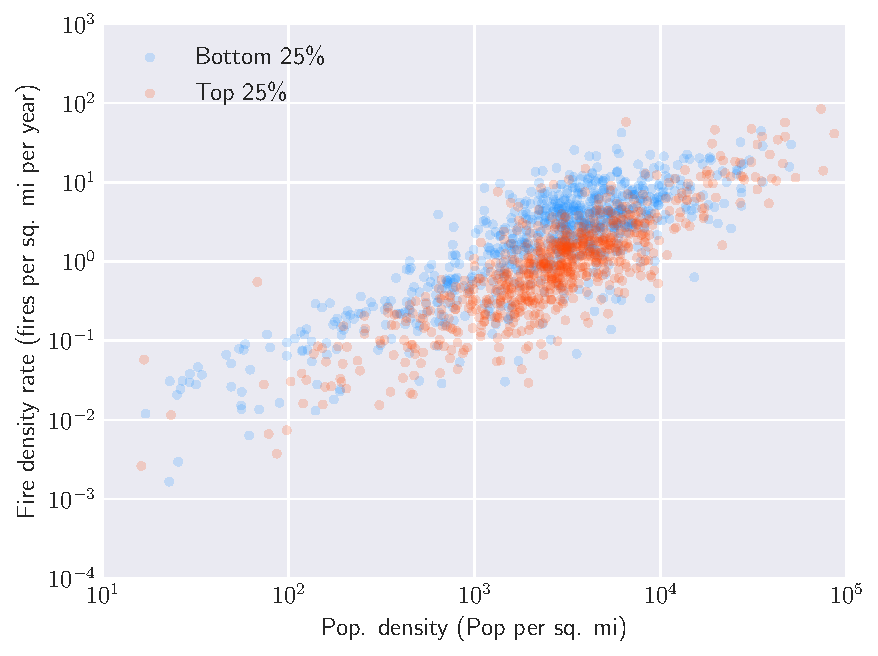
\includegraphics[width=.4\textwidth,keepaspectratio]{figures/frac_degree.pdf}
          }\\ % 
            \subfloat[Fraction of population that is Black]{%
             \label{fig:frac_black} 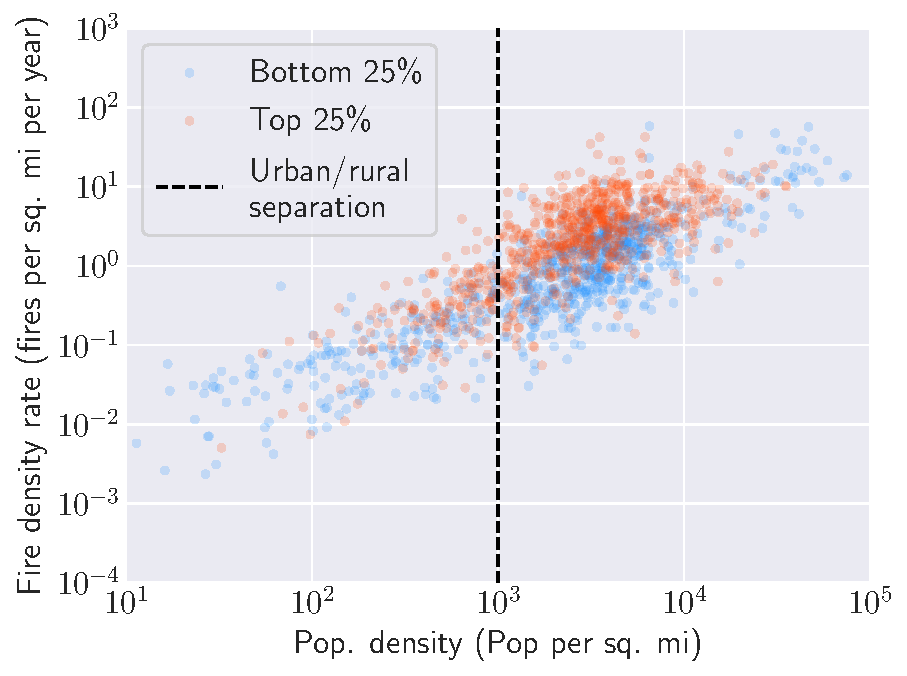
\includegraphics[width=.4\textwidth,keepaspectratio]{figures/frac_black.pdf}
          }
            \subfloat[Fraction of population that is White]{%
             \label{fig:frac_white} 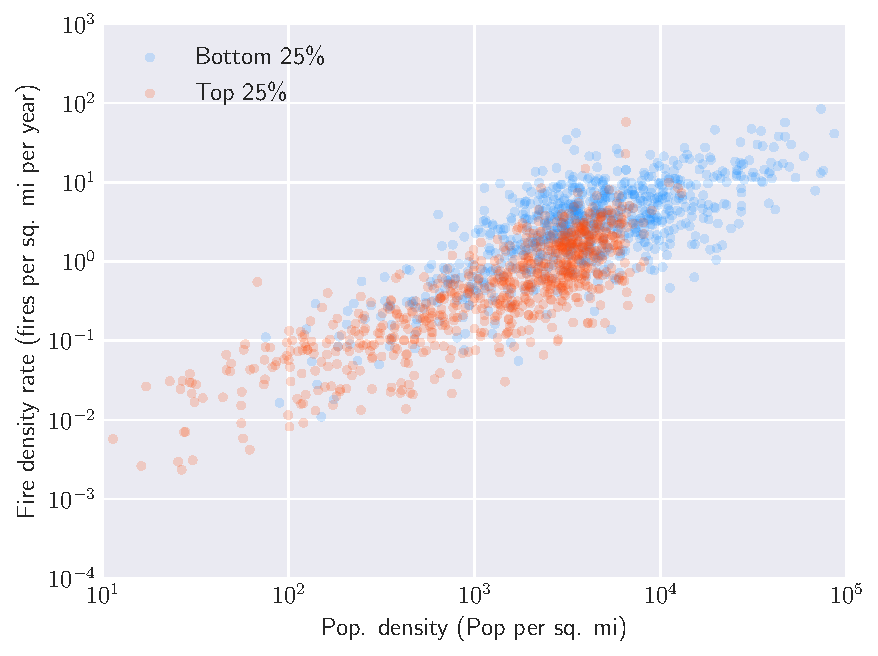
\includegraphics[width=.4\textwidth,keepaspectratio]{figures/frac_white.pdf}
          }\\
            \subfloat[Fraction of population that is Asian]{%
             \label{fig:frac_asian} 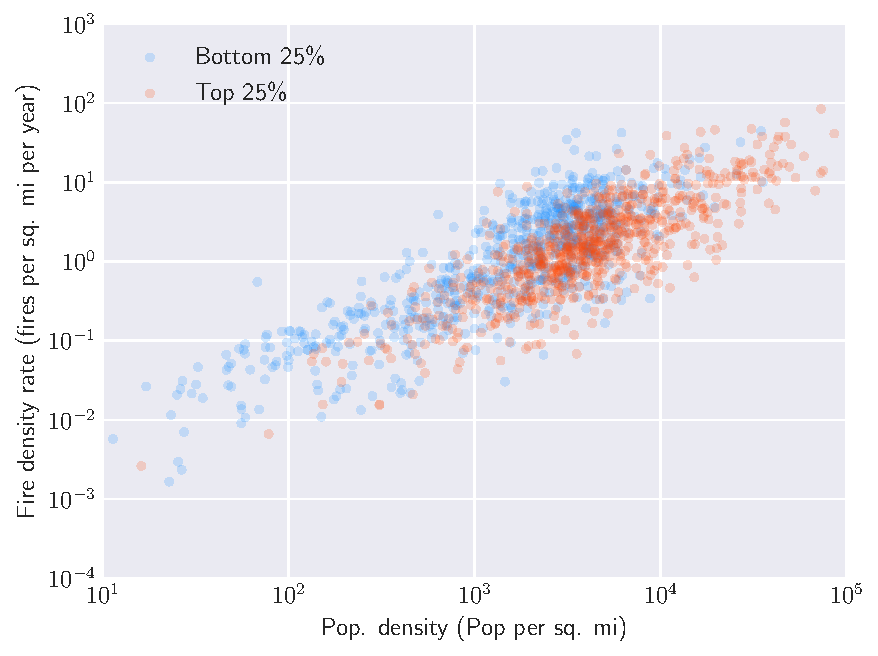
\includegraphics[width=.4\textwidth,keepaspectratio]{figures/frac_asian.pdf}
          }
            \subfloat[Fraction of population that is Hispanic]{%
             \label{fig:frac_hispanic} 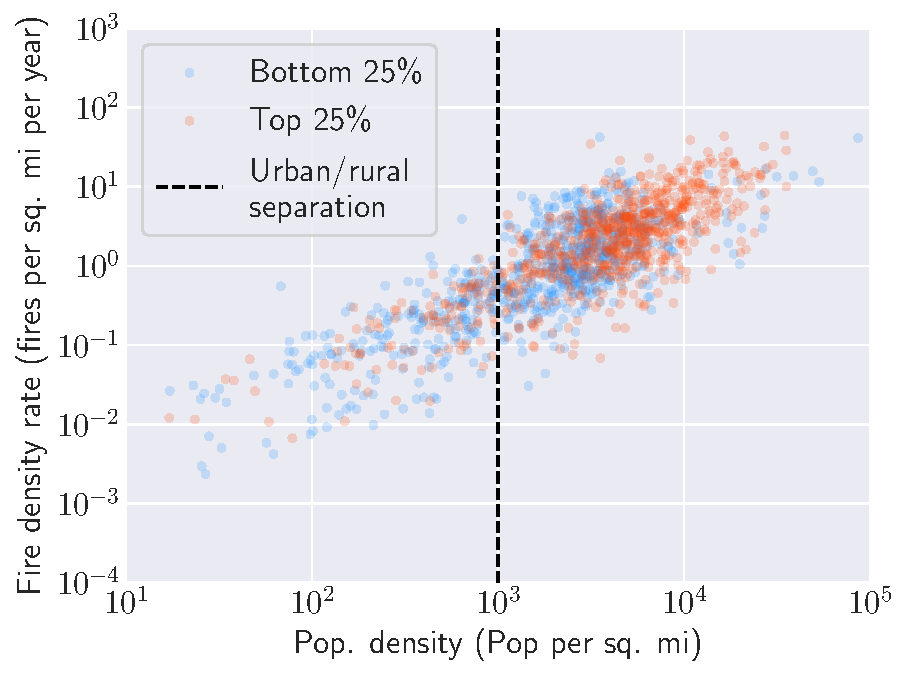
\includegraphics[width=.4\textwidth,keepaspectratio]{figures/frac_hispanic.pdf}
          }
      \end{center}
      \caption{Scatterplot of observed fire density rates ($\hat\Lambda_{count}$) during the training interval as a function of population density for census tracts in the top quartile (red) and bottom quartile (blue) of the specified sociodemographic quantities. For example, in \protect\subref{fig:median_income}, the red dots represent census tracts with median incomes in the top 25\% of all tracts in the dataset. Conversely, the blue dots represent census tracts with median incomes in the bottom 25\% of all census tracts in the dataset.}
     \label{fig:sociodemographic}
  \end{figure}
 
 
 These visualizations give insight into the populations who are most at risk for residential fires. Figures \ref{fig:median_income} and \ref{fig:frac_degree} show the expected result that census tracts with educated and high earning populations experience fires at a lower rate than those with low income or less educated populations. Interestingly, the relationship within the top and bottom quartiles of these quantities still appears linear, but the effect of increased socioeconomic status appears to shift the linear trend downward in the log-log plots. The effects of the racial and ethnic compositions shown in Figures \ref{fig:frac_black}-\ref{fig:frac_hispanic} show similar trends, which is likely due to the fact that these quantities are correlated with the socioeconomic factors shown in Figures \ref{fig:median_income} and \ref{fig:frac_degree}. 
 
Figure \ref{fig:building age} gives insight into the effect of building age on the fire frequency. The visualizations show the expected result that residential fires are more likely to occur in older buildings than newer ones. Interestingly, the census tracts with the highest fractions of buildings built before 1950 appear mostly in urbanized areas in the dataset, yet the cloud of points comprised of these census tracts appears to lie slightly above that comprised of the census tracts with fractions of buildings built before 1950 in the bottom quartile. Conversely, census tracts with a large fraction of housing units built more recently than 1990 have lower population densities and a slightly lower fire risk per person as well.

   \begin{figure}[!ht]
       \begin{center}
  %
          \subfloat[Fraction of housing units built before 1950]{%
              \label{fig:frac_1950} 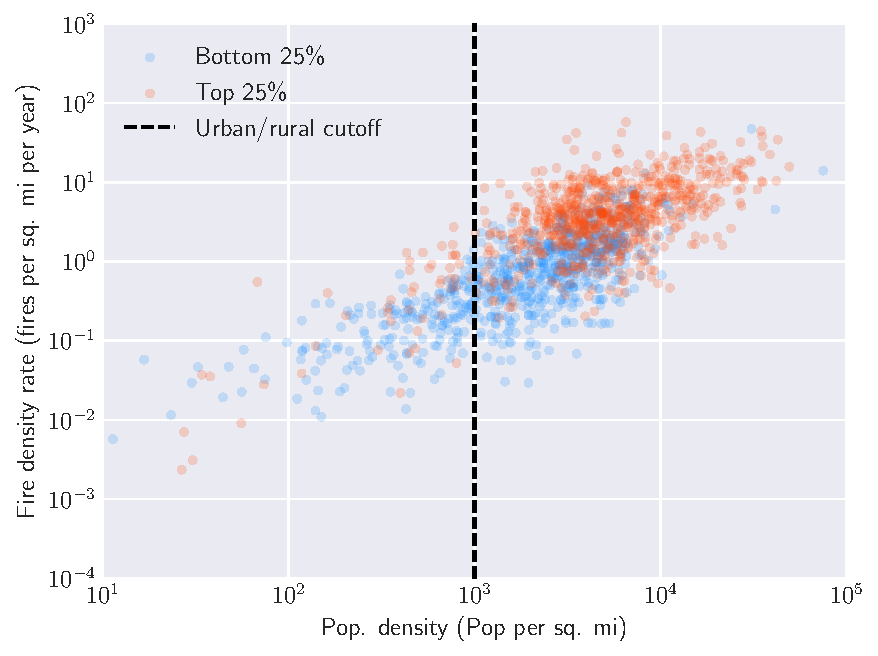
\includegraphics[width=.4\textwidth,keepaspectratio]{figures/frac_1950.pdf}
          }%
          \subfloat[Fraction of housing units built between 1950 and 1969]{%
             \label{fig:frac1950_1969} 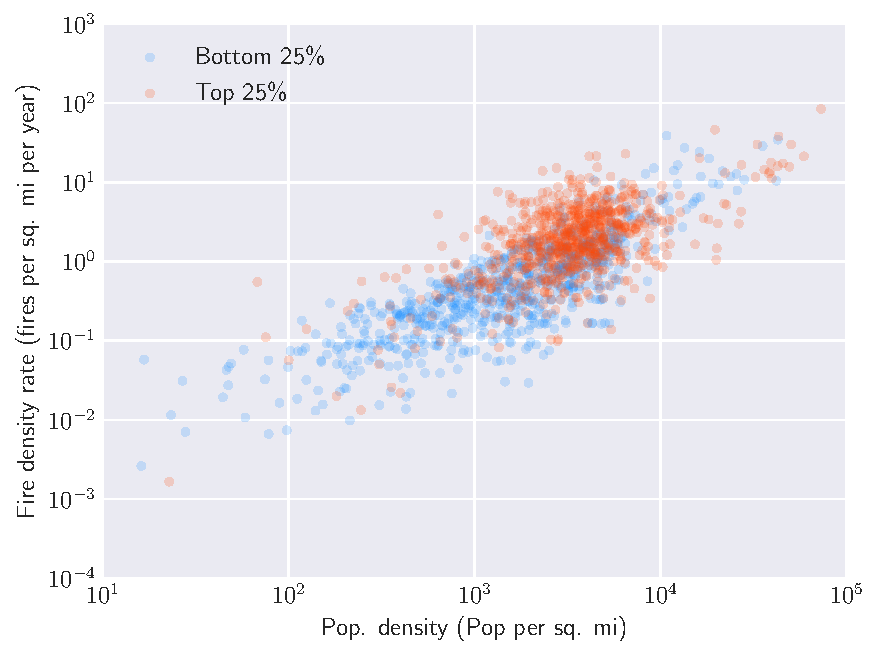
\includegraphics[width=.4\textwidth,keepaspectratio]{figures/frac_1950_1969.pdf}
          }\\ % 
            \subfloat[Fraction of housing units built between \newline 1970 and 1989]{%
             \label{fig:frac_1970_1989} 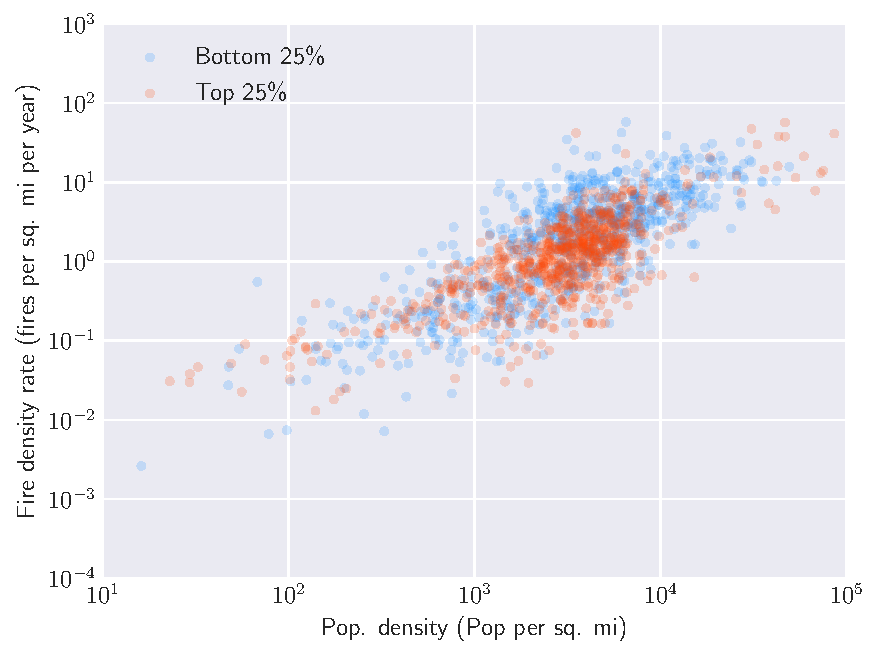
\includegraphics[width=.4\textwidth,keepaspectratio]{figures/frac_1970_1989.pdf}
          }
            \subfloat[Fraction of housing units built in 1990 or later]{%
             \label{fig:frac_1990} 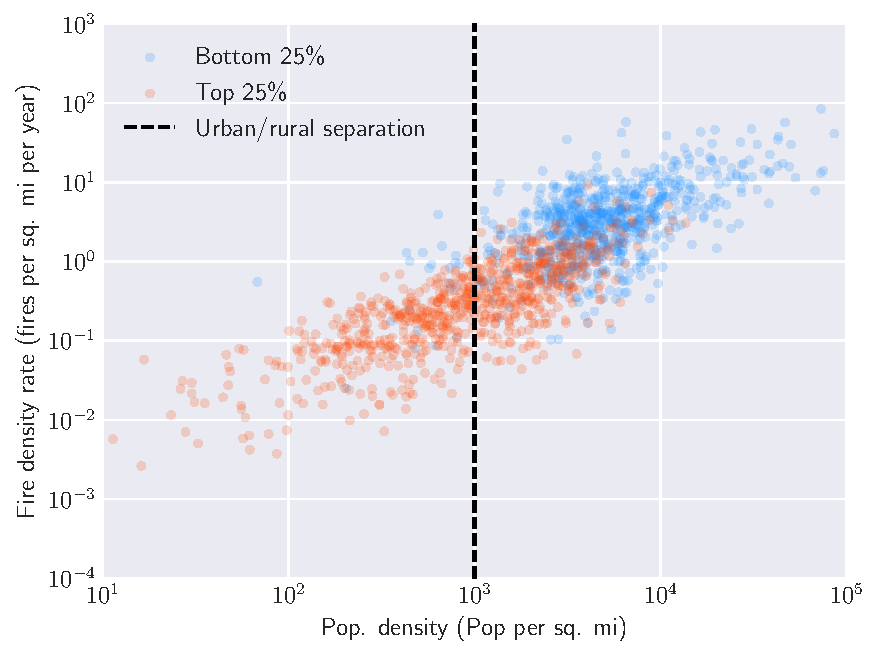
\includegraphics[width=.4\textwidth,keepaspectratio]{figures/frac_1990.pdf}
          }\\
          
      \end{center}
      \caption{Scatterplot of observed fire density rates ($\hat\Lambda_{count}$) during the training interval as a function of population density for census tracts in the top quartile (red) and bottom quartile (blue) of the specified quantity relating to structure age. For example, in \protect\subref{fig:frac_1950}, the red dots represent census tracts with fractions of housing units built before 1950 in the top 25\% of all tracts in the dataset. Conversely, the blue dots represent census tracts with fractions of housing units built before 1950 in the bottom 25\% of all census tracts in the dataset.}
     \label{fig:building age}
  \end{figure}
 
    Lastly, Figure \ref{fig:occupancy} gives insight into the effect of different occupancy characteristics on residential fire risk. Again, the expected trends appear- the fire risk appears to be greater in census tracts with higher fractions of renter-occupied housing compared to owner-occupied housing. Also, the differences in these features is correlated with population density with the top quartile of renter-occupied census tracts are mostly urbanized. Large fractions of housing on fire risk per person shown in Figure \ref{fig:frac_vacant} also appears to elevate the residential fire risk per person,  but the top quartile appears to have more variability in the fire risk per person than the bottom quartile. Not surprsingly, census tracts with large fractions of single-unit housing follows similar trends as those with high fractions of owner occupied units. 
 
   \begin{figure}[!ht]
       \begin{center}
  %
          \subfloat[Fraction of housing units occupied \newline by a renter]{%
              \label{fig:frac_rented} 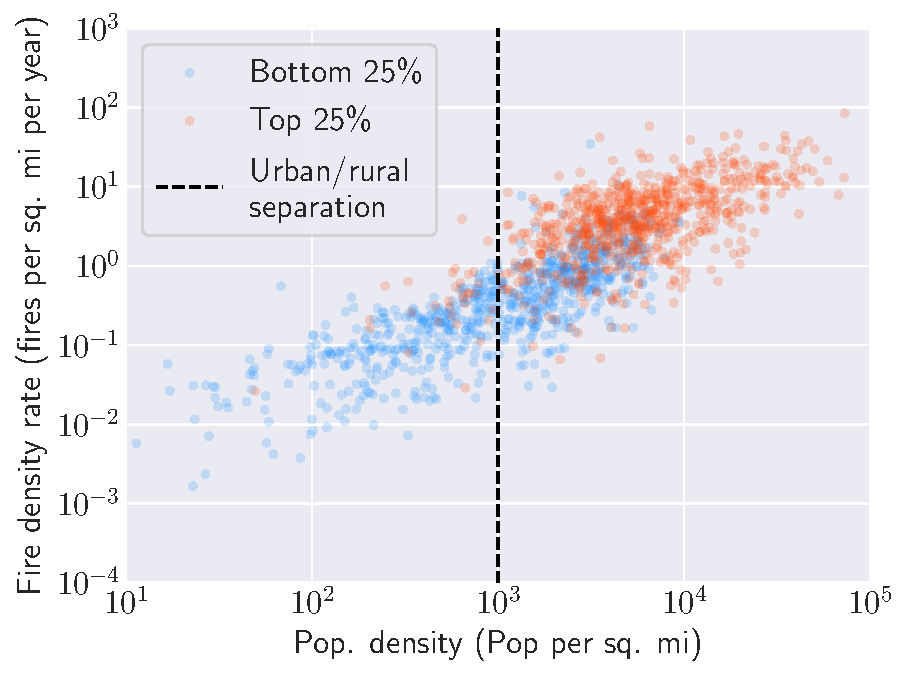
\includegraphics[width=.4\textwidth,keepaspectratio]{figures/frac_rented.pdf}
          }%
          \subfloat[Fraction of housing units occupied by the owner]{%
             \label{fig:frac_owner} 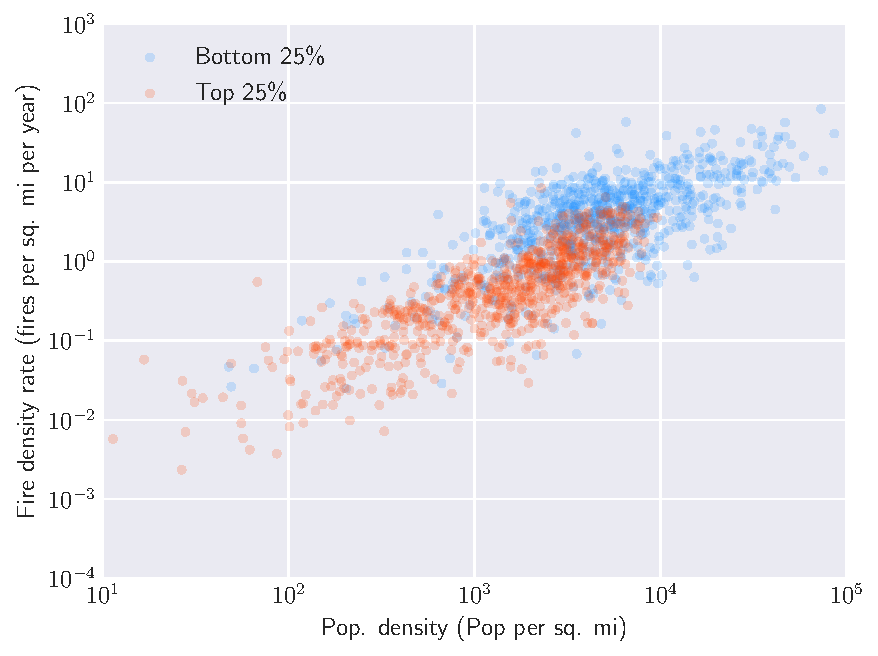
\includegraphics[width=.4\textwidth,keepaspectratio]{figures/frac_owner.pdf}
          }\\ %           
          \subfloat[Fraction of housing units that are vacant ]{%
             \label{fig:frac_vacant} 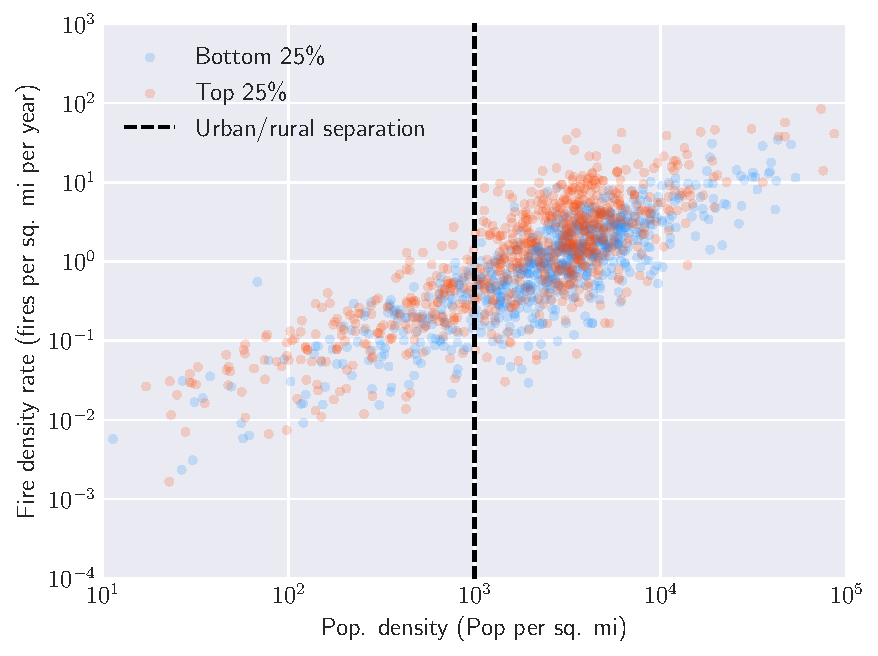
\includegraphics[width=.4\textwidth,keepaspectratio]{figures/frac_vacant.pdf}
          } % 
            \subfloat[Fraction of housing units that are single (not apartments)]{%
             \label{fig:frac_1_unit} 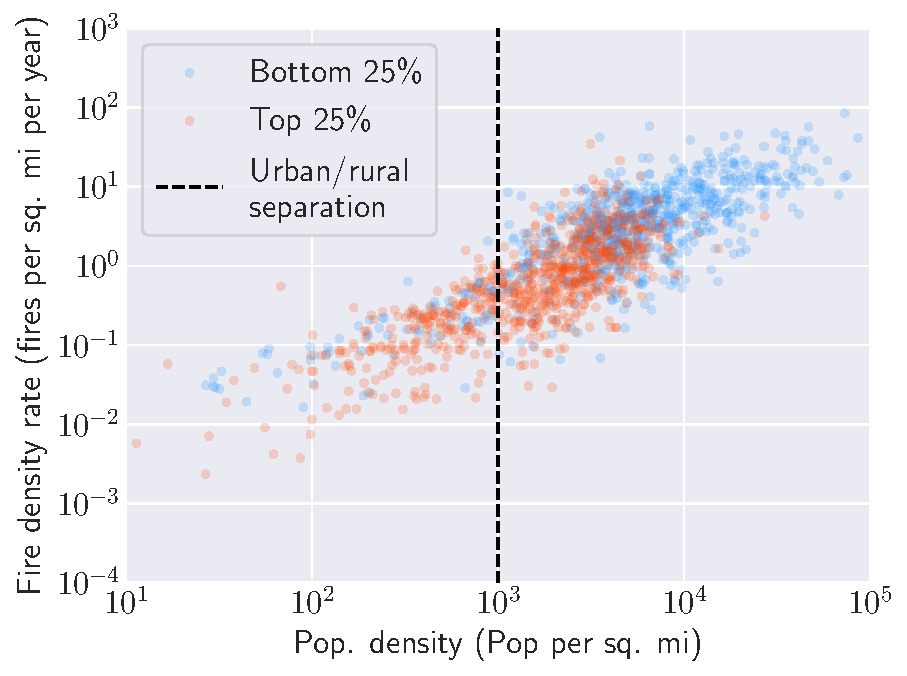
\includegraphics[width=.4\textwidth,keepaspectratio]{figures/frac_1_unit.pdf}
          }
      \end{center}
      \caption{Scatterplot of observed fire density rates ($\hat\Lambda_{count}$) during the training interval as a function of population density for census tracts in the top quartile (red) and bottom quartile (blue) of the specified quantity relating to occupancy. For example, in \protect\subref{fig:frac_rented}, the red dots represent census tracts with fractions of housing units occupied by a renter in the top 25\% of all tracts in the dataset. Conversely, the blue dots represent census tracts with fractions of housing units occupied by a renter in the bottom 25\% of all census tracts in the dataset.}
     \label{fig:occupancy}
  \end{figure}
 
 
 \clearpage
  \subsubsection{A hierarchical Bayesian Poisson regression model}
  The feature visualizations presented in the previous section motivated the use of a Bayesian Poisson regression model. However, because some of the ACS5 variables are correlated, a principal components analysis (PCA) was conducted to reduce the number of feature variables. This is a statistical technique that utilizes correlations between input variables to reduce the dimensionality of the dataset. This is done by projecting the input data into a new space where certain dimensions can be disregarded while still retaining most of the variation of the original dataset. The projection vectors are the eigenvectors of the covariance matrix of feature variables and the transformed features are linearly uncorrelated. A simple example of this technique is illustrated in \ref{fig:pca}.
  
    \begin{figure}[!htb]
       \begin{center}
  %
          \subfloat[Layout of census tracts]{%
              \label{fig:tract_layout} 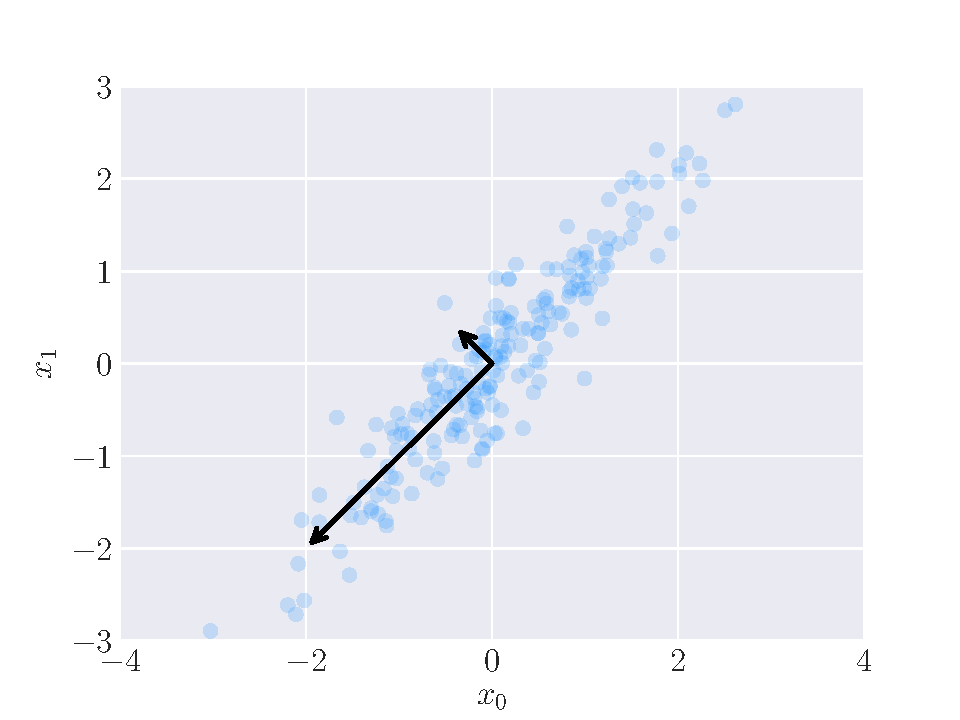
\includegraphics[width=.4\textwidth,keepaspectratio]{figures/pca_raw.pdf}
          }%
          \subfloat[Distance matrix based on neighbors]{%
             \label{fig:distance_mat} 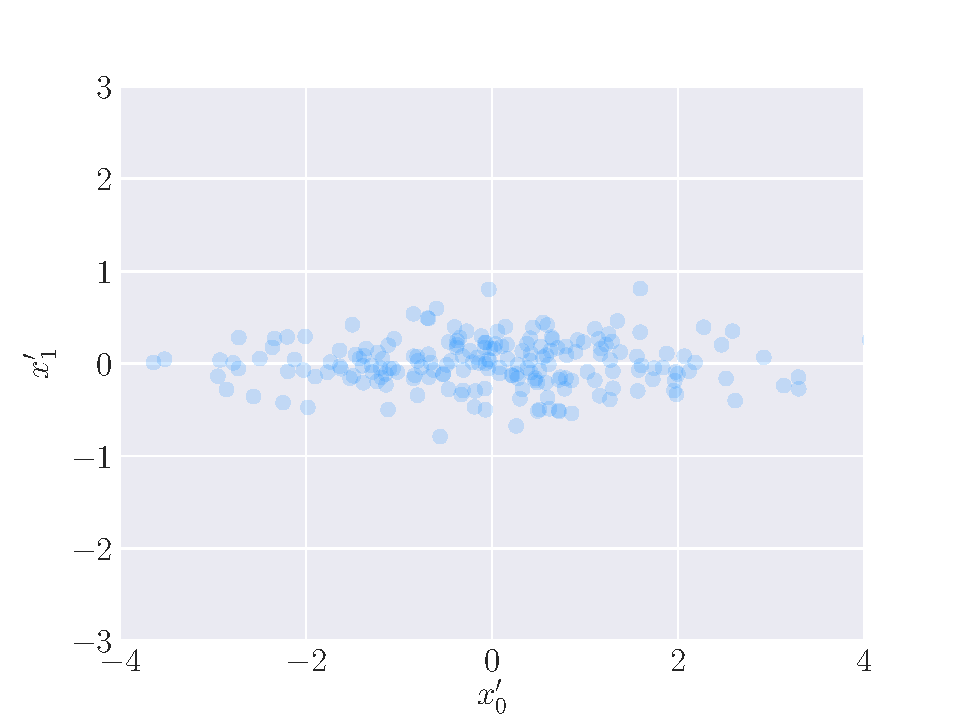
\includegraphics[width=.45\textwidth,keepaspectratio]{figures/pca_projected.pdf}
          } %           
      \end{center}
      \caption{An example of the resulting distance matrix for a department}
     \label{fig:pca}
  \end{figure}
  
  
  
  
  
  
  
  
  \subsection{Combining spatial, structural, and demographic information}
  
  
  
\begin{figure}[htb] \centering
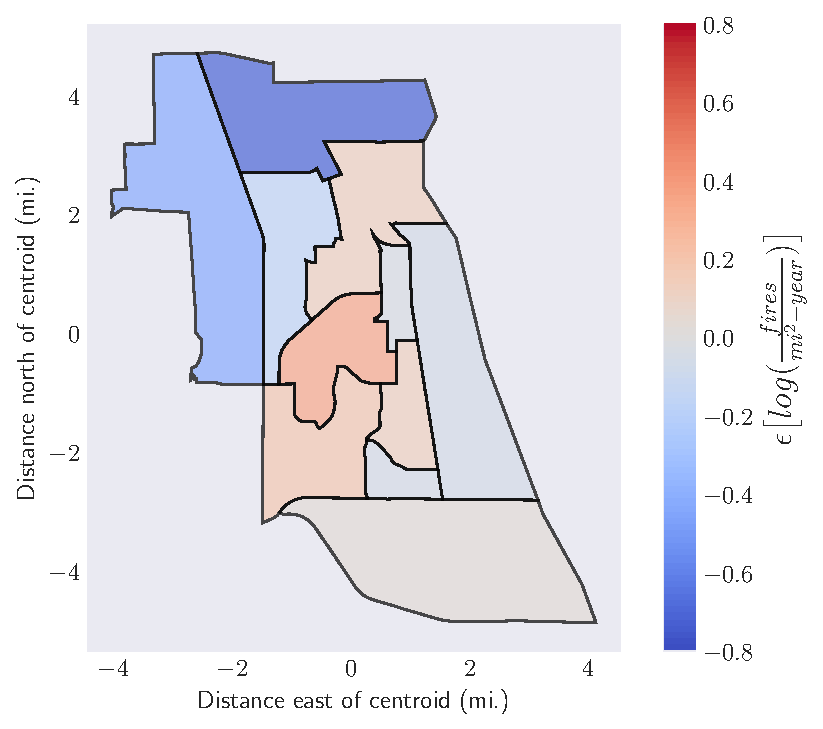
\includegraphics[width=.75\textwidth]{figures/spatial_correlation.pdf}
\caption{SPATIAL CORRELATION}
\label{fig:spatialcorr}
\end{figure}

  
  \begin{figure}[!htb]
       \begin{center}
  %
          \subfloat[Layout of census tracts]{%
              \label{fig:tract_layout} 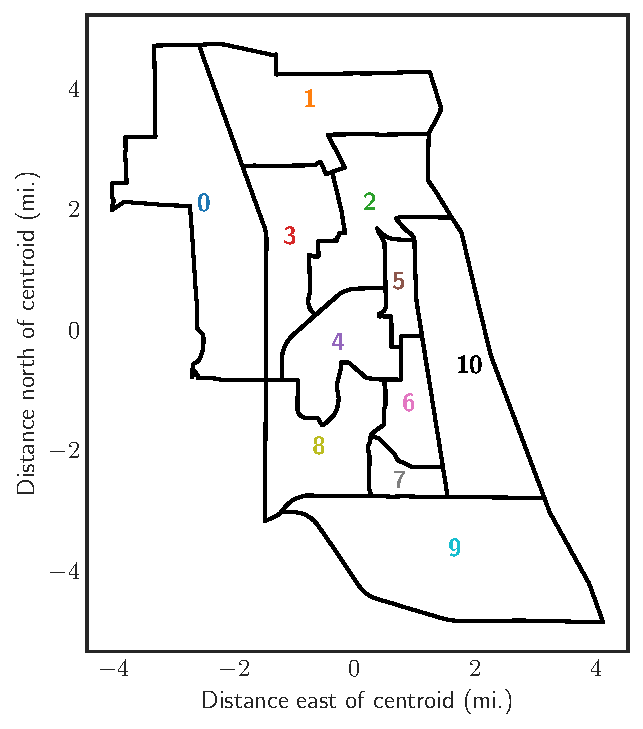
\includegraphics[width=.4\textwidth,keepaspectratio]{figures/tract_num.pdf}
          }%
          \subfloat[Distance matrix based on neighbors]{%
             \label{fig:distance_mat} 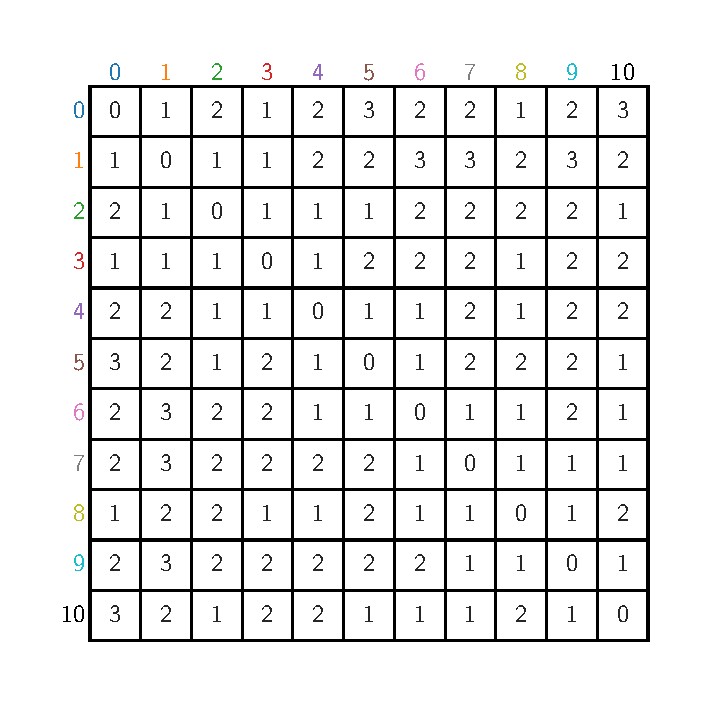
\includegraphics[width=.45\textwidth,keepaspectratio]{figures/sep_matrix.pdf}
          } %           
      \end{center}
      \caption{An example of the resulting distance matrix for a department}
     \label{fig:sep_example}
  \end{figure}
  
  
  
  
  
  
 \section{Model evaluation and comparison}
  
    \begin{table}[htb] \centering
    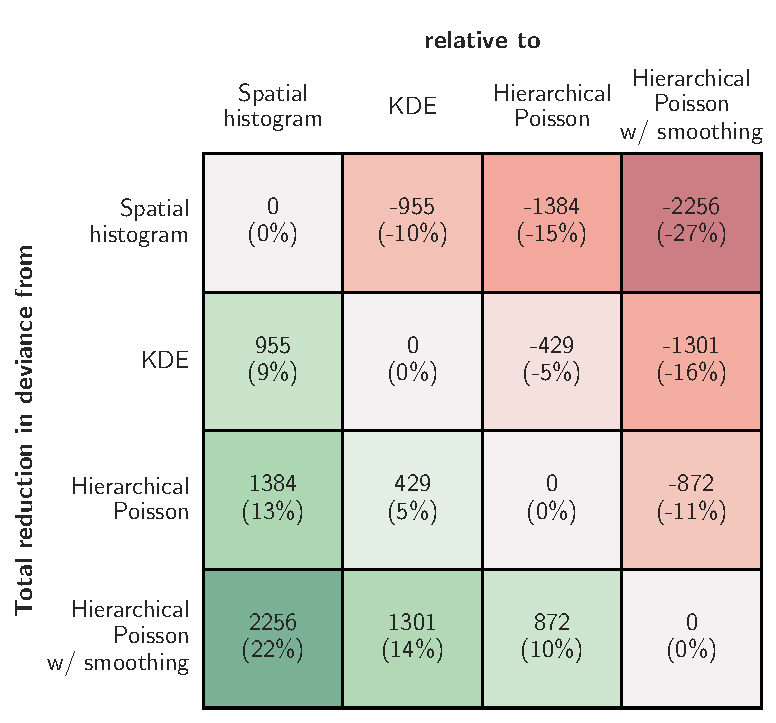
\includegraphics[width=.75\textwidth]{figures/dev_table.pdf}
    \caption{A }
    \label{table:dev_table}
    \end{table}
  
    \begin{table}[htb] \centering
    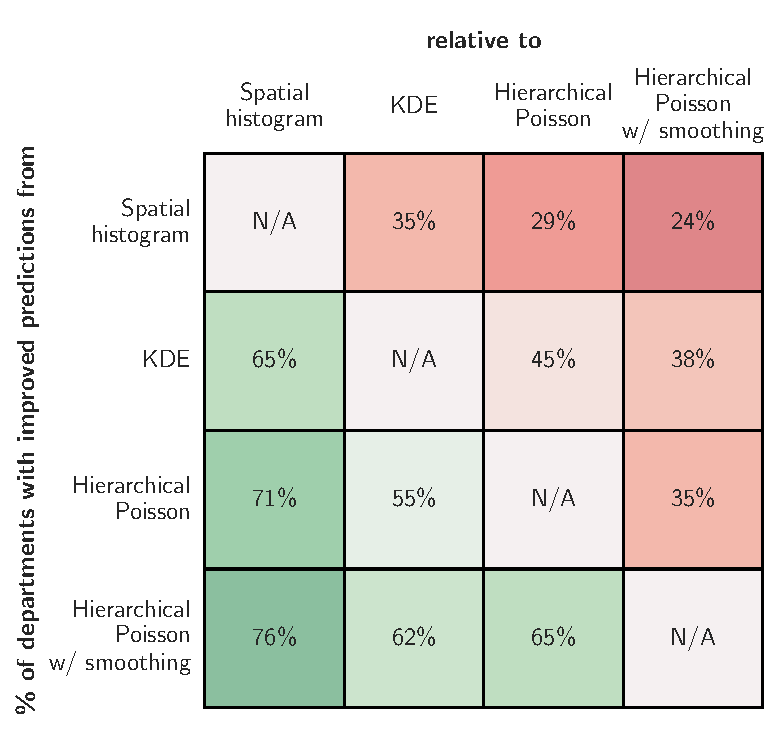
\includegraphics[width=.75\textwidth]{figures/department_comparison.pdf}
    \caption{A}
    \label{table:dep_comparison}
    \end{table}
  
  
  
    \begin{figure}[htb] \centering
    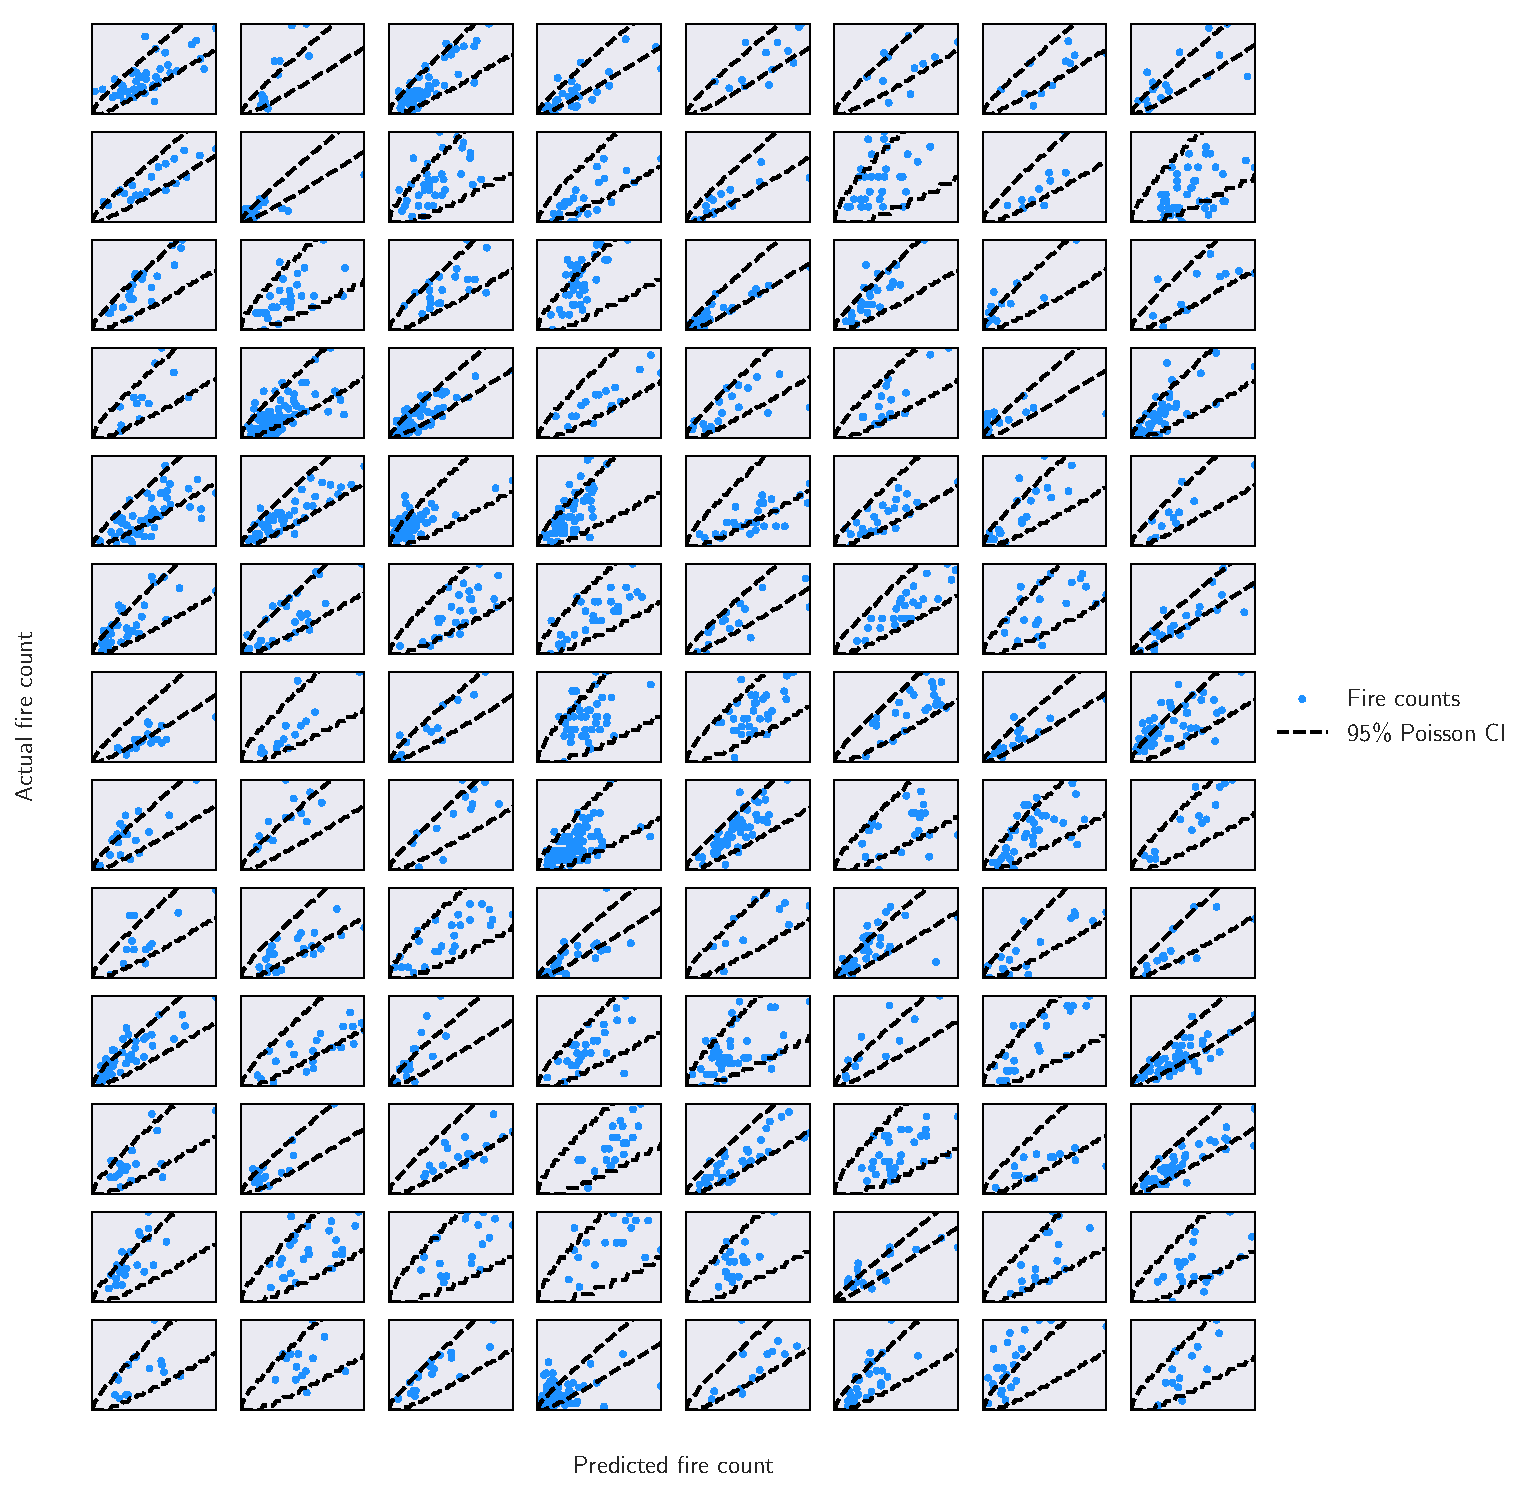
\includegraphics[width=1\textwidth]{figures/dispersion.pdf}
    \caption{A }
    \label{fig:dispersion}
    \end{figure}
  
  
  
  
  
  \section{Conclusions}
  

\clearpage
\bibliographystyle{unsrtnat}
\bibliography{./references.bib}
\end{document}
